\documentclass[pdf]{beamer}
\mode<presentation>{}

%\usetheme{UniversiteitGent}

\usepackage{array}
\usepackage{varwidth}
\usepackage{multirow}
\usepackage{color}

\newcolumntype{M}{>{\begin{varwidth}{4cm}}l<{\end{varwidth}}} %M is for Maximal column

%Define my own footer here
\setbeamertemplate{footline}[text line]{%
  \parbox{\linewidth}{\vspace*{-8pt}\insertsection\hfill\insertshortauthor\hfill\insertpagenumber}}
\setbeamertemplate{navigation symbols}{}

%%Defining some nice colors
\definecolor{olive}{rgb}{0.3, 0.4, .1}
\definecolor{fore}{RGB}{249,242,215}
\definecolor{back}{RGB}{51,51,51}
\definecolor{title}{RGB}{255,0,90}
\definecolor{dgreen}{rgb}{0.,0.6,0.}
\definecolor{gold}{rgb}{1.,0.84,0.}
\definecolor{JungleGreen}{cmyk}{0.99,0,0.52,0}
\definecolor{BlueGreen}{cmyk}{0.85,0,0.33,0}
\definecolor{RawSienna}{cmyk}{0,0.72,1,0.45}
\definecolor{Magenta}{cmyk}{0,1,0,0}

%%Useful physics symbols
\newcommand{\dzero}{D\O\ }
\newcommand{\invpb}{$\rm{pb}^{-1}$}
\newcommand{\invfb}{$\rm{fb}^{-1}$}
\newcommand{\ttbar}{\mbox{${t\bar{t}}$}}
\newcommand{\bbbar}{\mbox{${b\bar{b}}$}}
\newcommand{\ppbar}{\mbox{${p\bar{p}}$}}
\newcommand{\qqbar}{\mbox{${q\bar{q}}$}}
\newcommand{\llbar}{\mbox{${l\bar{l}}$}}
\newcommand{\pt}{\mbox{${p_T}$}}
\newcommand{\mll}{\mbox{$m_{\ell\ell}$}}
\newcommand{\ptrel}{\mbox{${p_{Trel}}$}}
\newcommand{\herwig}    {{\sc herwig }}
\newcommand{\pythia}    {{\sc pythia }}
\newcommand{\vecbos}    {{\sc vecbos }}
\newcommand{\alpgen}    {{\sc alpgen }}
\newcommand{\qq}        {{\sc qq }}
\newcommand{\tauola}    {{\sc tauola }}
\newcommand{\geant}     {{\sc geant }}
\newcommand{\met}       {\mbox{$\not\!\!E_{{T}}$}}
\newcommand{\metrel}       {\mbox{$\not\!\!E_{{T}}^{Rel}$}}
\newcommand{\mpt}       {\mbox{$\not\!p_{{T}}$}}
\newcommand{\mptvec}       {\mbox{$\not\!\overrightarrow{p_{T}}$}}
\newcommand{\metcal}    {\mbox{$\not\!\!E_{{Tcal}}$ }}
\newcommand{\metscaled}    {\mbox{$\not\!\!E_{{T}}^{Scaled}$ }}
\newcommand{\ki}    {\mbox{$\chi^2$}}
\newcommand{\vo}    {\mbox{$V^0$}}
\newcommand{\kshort}    {\mbox{$K^0_S$}}
\newcommand{\GeVcc}{\mbox{${\rm GeV}/c^2$}}
\newcommand{\GeVc}{\mbox{${\rm GeV}/c$}}
\newcommand{\MeVcc}{\mbox{${\rm MeV}/c^2$}}
\newcommand{\MeVc}{\mbox{${\rm MeV}/c$}}
\newcommand{\HT}    {\mbox{${H_T}$}}
\newcommand{\ET}    {\mbox{${E_T}$}}
\newcommand{\lplus}    {\mbox{$\mathbf{\ell +}$}}
\newcommand{\ljets}    {\mbox{$\mathbf{\ell + jets}$}}
\newcommand{\aplanarity}    {\mbox{$\mathcal{A}$}}
\newcommand{\epsqcd}    {\mbox{$\varepsilon_{QCD}$}}
\newcommand{\epssig}    {\mbox{$\varepsilon_{sig}$}}
\newcommand{\pf} {\phantom{5}}
\newcommand{\ppf} {\phantom{.5}}
\newcommand{\data} {Data}
\newcommand{\smWW} {$WW\rightarrow\ell\nu\ell\nu$}
\newcommand{\smW} {$W\rightarrow\ell\nu$}
\newcommand{\smZ} {$Z\rightarrow\ell\ell$}
\newcommand{\smEW} {Diboson}
\newcommand{\sTop} {Single Top}
\newcommand{\higgs} {Higgs}
\newcommand{\hOneFifty} {Higgs (150GeV)}
\newcommand{\totalBack} {Total MC}
\newcommand{\e}[1]{\ensuremath{\times 10^{#1}}}


%%preamble
\title{How Many Bikes are Needed?}
\subtitle{Exploratory Analysis and Regression of a Bike Sharing Dataset}
\author[S.Crucy]{Shannon Crucy \\%[\baselineskip]
}
\date{\today}
%\institute{Ghent University}

\defbeamertemplate*{title page}{customized}[1][]
{
\usebeamerfont{title}\inserttitle\par
\usebeamerfont{subtitle}\usebeamercolor{subtitle}\insertsubtitle\par
\bigskip
\usebeamerfont{author}\insertauthor\par
\usebeamerfont{institute}\insertinstitute\par
\usebeamerfont{date}\insertdate\par
}

\begin{document}
%%%%%%%%%%%%%%%%%%%%%%%%%%%%%%%%%%%%%%%%%%%%%%%%%%%%%%%

\begin{frame}
\titlepage
\end{frame}

%%%%%%%%%%%%%%%%%%%%%%%%%%%%%%%%%%%%%%%%%%%%%%%%%%%%%%%

\begin{frame}{Overview and Dataset}
\begin{itemize}
\item{These slides summarize an exploratory analysis of a bike-sharing dataset, including developing a prediction model for the total number of rented bikes.}
\item{The dataset contains information on the rental of bikes per hour by Captial Bikeshare system, Washington D.C., USA in the years 2011 and 2012.  It contains 17379 records.}
\item{Outline:}
\begin{itemize}
\item{Available Features}
\item{The Models}
\item{Conclusions}
\end{itemize}
\end{itemize}
\end{frame}

%%%%%%%%%%%%%%%%%%%%%%%%%%%%%%%%%%%%%%%%%%%%%%%%%%%%%%%

\begin{frame}{Available Features}
\begin{itemize}
\item{Information available in the dataset:}
\begin{center}
\scalebox{0.7}{
\begin{tabular}{l|l}
Date & Temperature \\
Season & Perceived Temperature\\
Year & Humidity \\
Month & Windspeed \\
Hour & Number of Weather situation \\
Holiday flag & Number of Registered Users \\
Workingday flag & Number of Casual Users \\
Day of Week & Total number of rented bikes \\
\end{tabular}
}
\end{center}
\small
\item{Note: $Total number of rented bikes = Registered Users + Casual Users$.  As the goal is to predict the total number of rented bikes, presumably somewhat in advance, the number of registered and casual users would not be available nor be a good input feature.}
\item{The exact date will also be omitted as containing a high level of overlapping information with the year, month, and weekday fields.}
\end{itemize}
\end{frame}

%%%%%%%%%%%%%%%%%%%%%%%%%%%%%%%%%%%%%%%%%%%%%%%%%%%%%%%

\begin{frame}{Feature Selection}
\begin{columns}
\column{0.65\textwidth}
\begin{itemize}
\small
\item{The best features were determined by their linear correlation with the count of rented bikes (via sklearn's SelectKBest).  Algorithms were built on groups of the best six, best nine, and all twelve available input variables, to check for possible over-fitting due to insufficient amount of input data relative to the features used.}
\begin{center}
\scalebox{0.5}{
\begin{tabular}{|c|c|}
\hline
Best 6 & Best 9\\
\hline
Weekday & Weekday \\
Temperature & Temperature \\
Perceived Temperature & Perceived Temperature \\
Windspeed & Windspeed \\
Hour & Hour \\
Weather Situation & Weather Situation \\
 & Humidity \\
 & Working day flag \\
 & Year \\
\hline
\end{tabular}
}
\end{center}
\item{Visually, the variables related to hour, temperature, and windspeed have the strongest correlation with number of rented bikes (additional scatter plots for other variables in the back-up).}
\end{itemize}
\column{0.35\textwidth}
\begin{center}
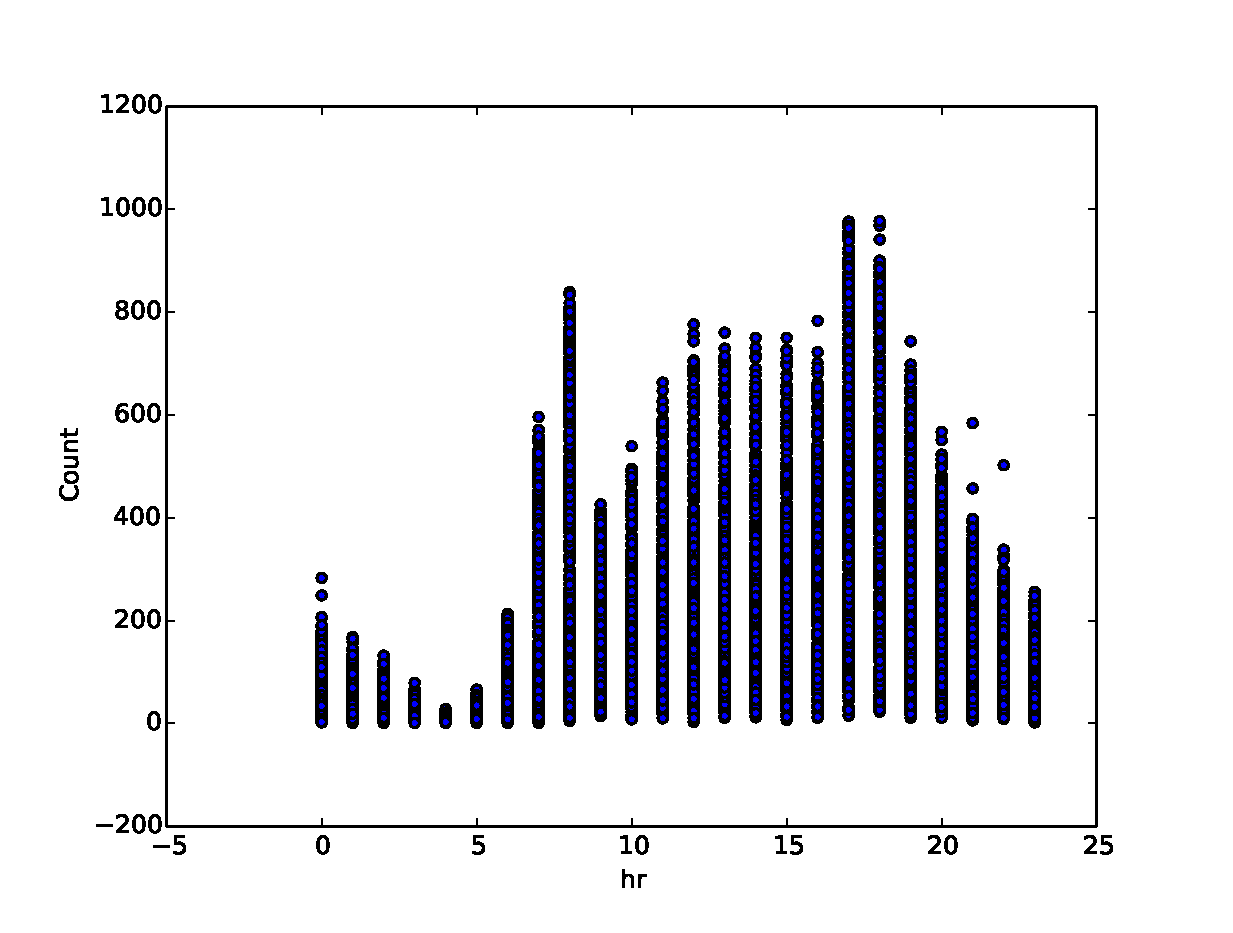
\includegraphics[width=0.9\textwidth]{plots/hr_v_Count_corrcheck.eps}\\
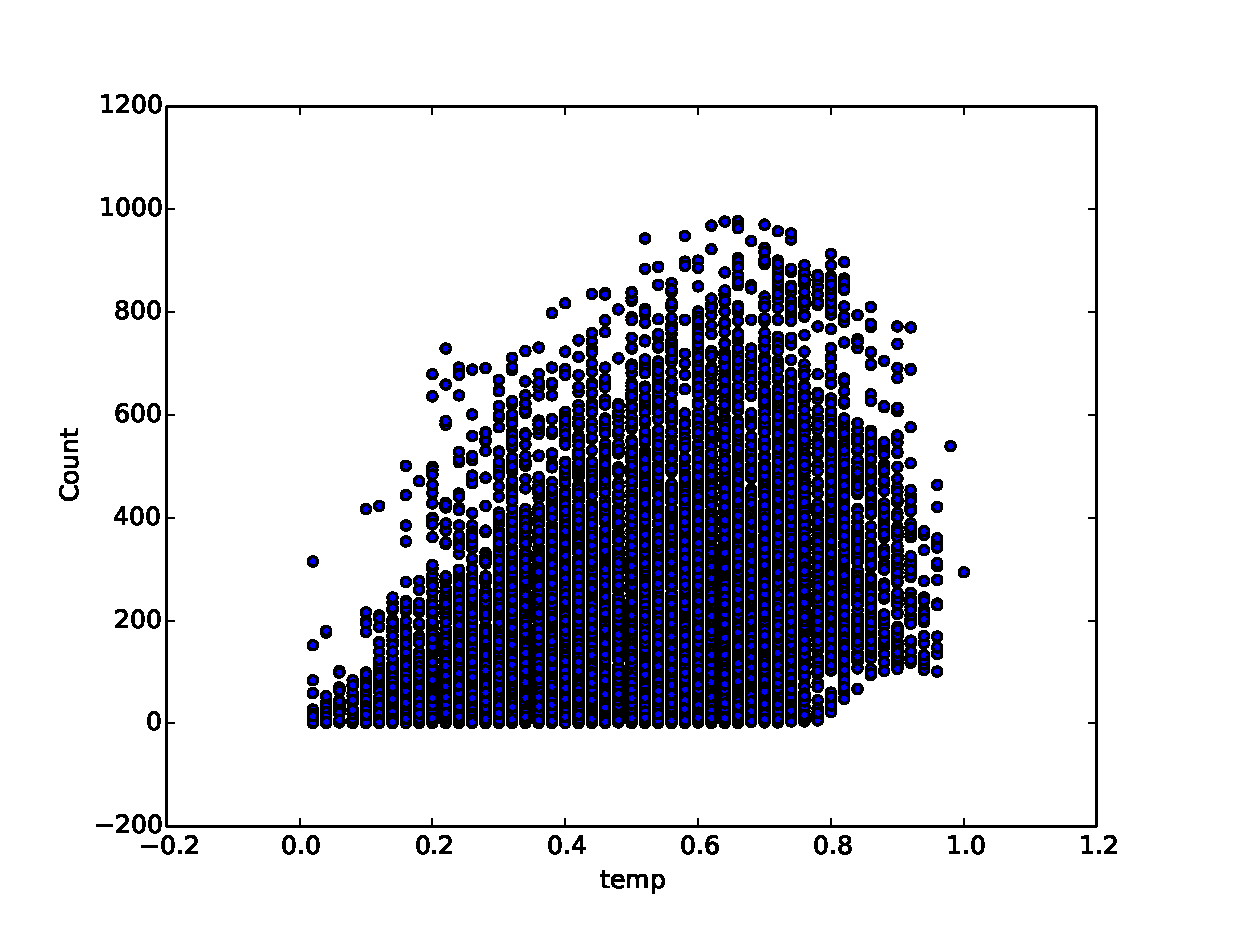
\includegraphics[width=0.9\textwidth]{plots/temp_v_Count_corrcheck.eps}\\
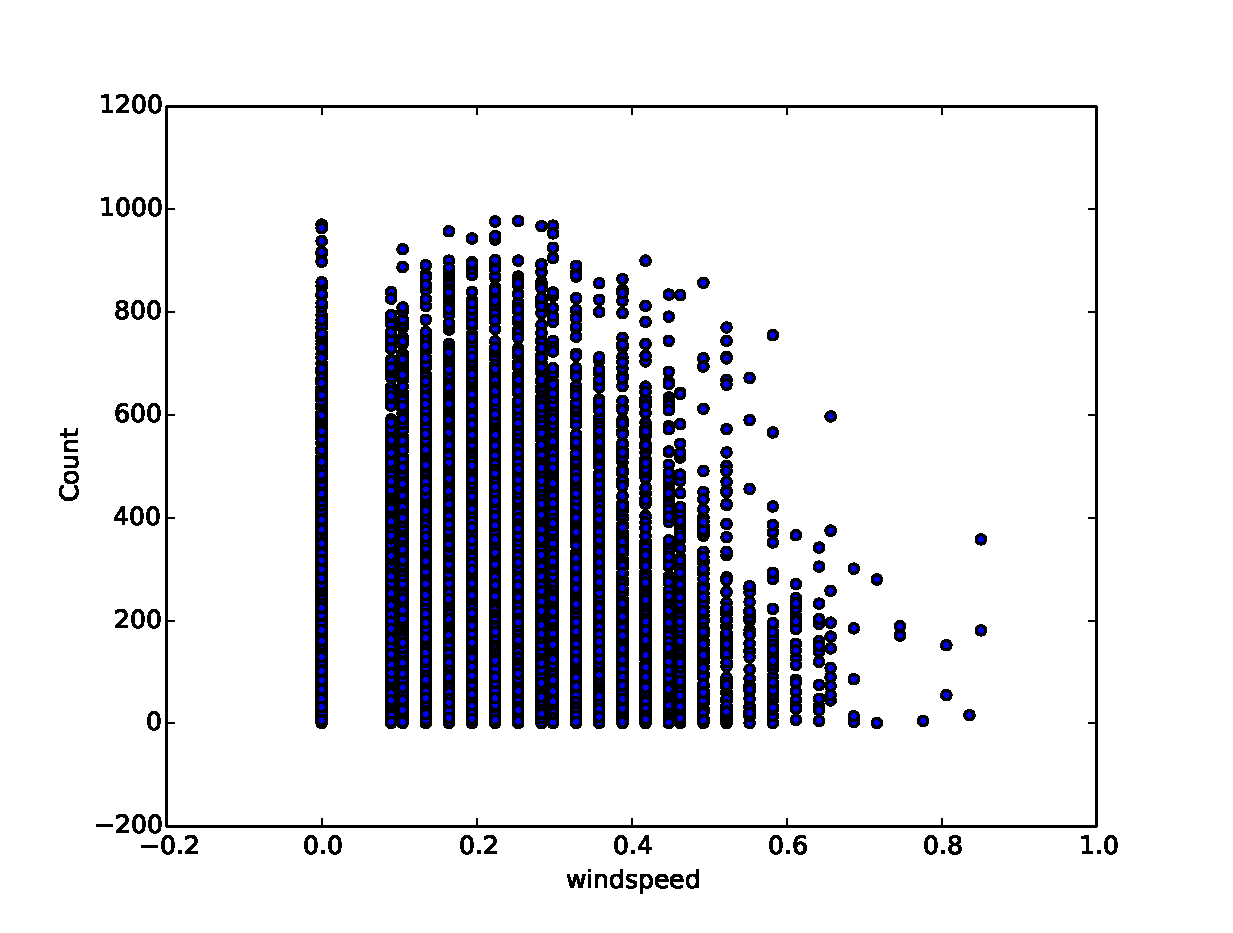
\includegraphics[width=0.9\textwidth]{plots/windspeed_v_Count_corrcheck.eps}
\end{center}
\end{columns}
\end{frame}

%%%%%%%%%%%%%%%%%%%%%%%%%%%%%%%%%%%%%%%%%%%%%%%%%%%%%%%

\begin{frame}{The Algorithms}
\begin{itemize}
\item{Lasso and Random Forest regression algorithms (as implemented in sklearn) were built on each set of input variables; these algorithms were selected for their resilience against weak input variables.  All features were scaled prior to training and a KFold of five was used.  The mean absolute error was used for comparison, and 10$\%$ of the input data was reserved for evaluation.}
\end{itemize}
\begin{columns}
\column{0.6\textwidth}{'Best Algorithm': Random Forest}
\begin{itemize}
\item{12 input features}
\item{100 estimators, minimum sample split of 6, maximum depth of 12}
\item{Best KFold score: -43.68$\pm$5.54}
\item{Global training score: -20.57}
\item{Evaluation score: -28.98} 
\end{itemize}
\column{0.4\textwidth}
\begin{center}
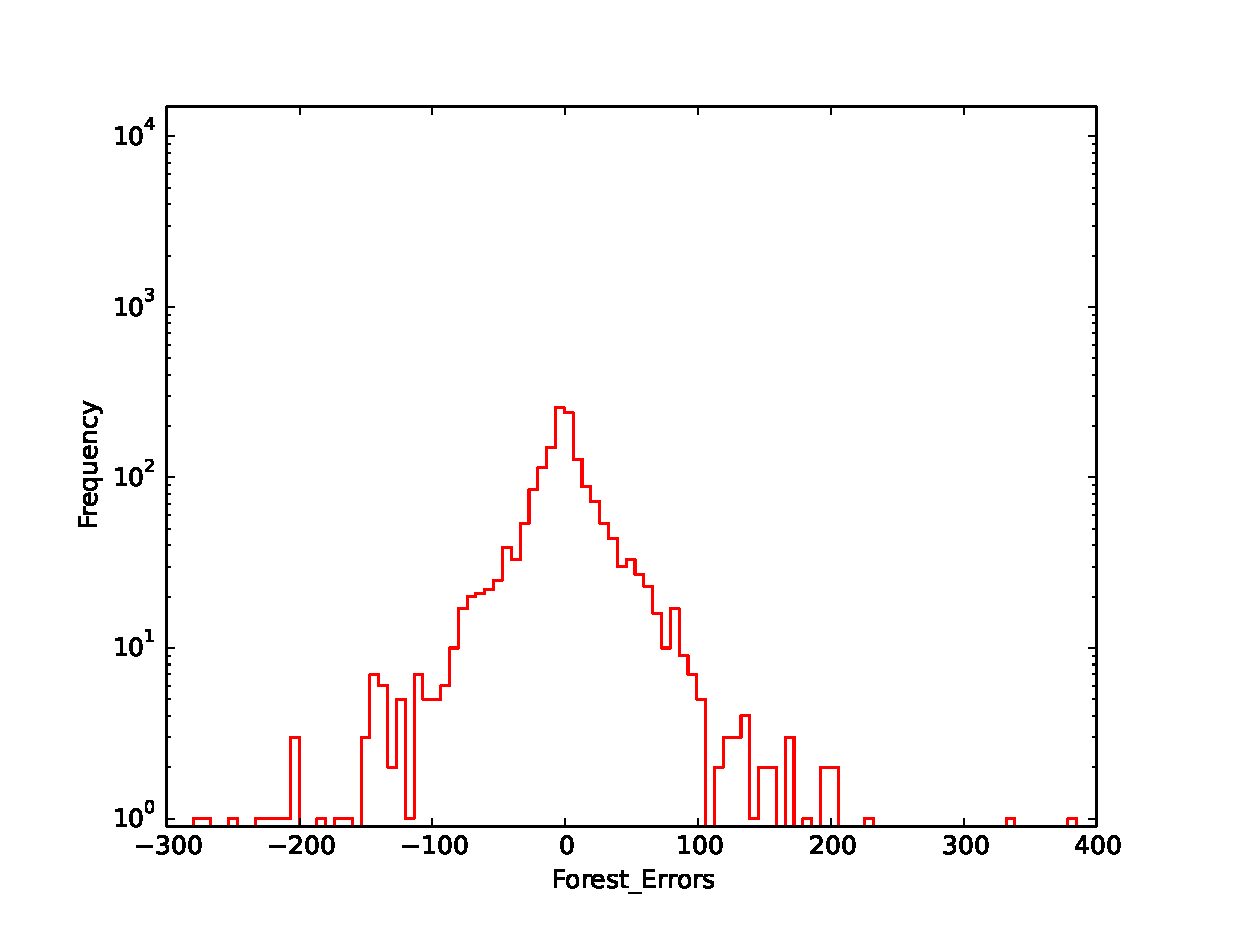
\includegraphics[width=1.05\textwidth]{plots/Forest_Errors_12.eps}
\end{center}
\end{columns}
\end{frame}

%%%%%%%%%%%%%%%%%%%%%%%%%%%%%%%%%%%%%%%%%%%%%%%%%%%%%%%

\begin{frame}{Lasso vs. Random Forest}
\begin{center}
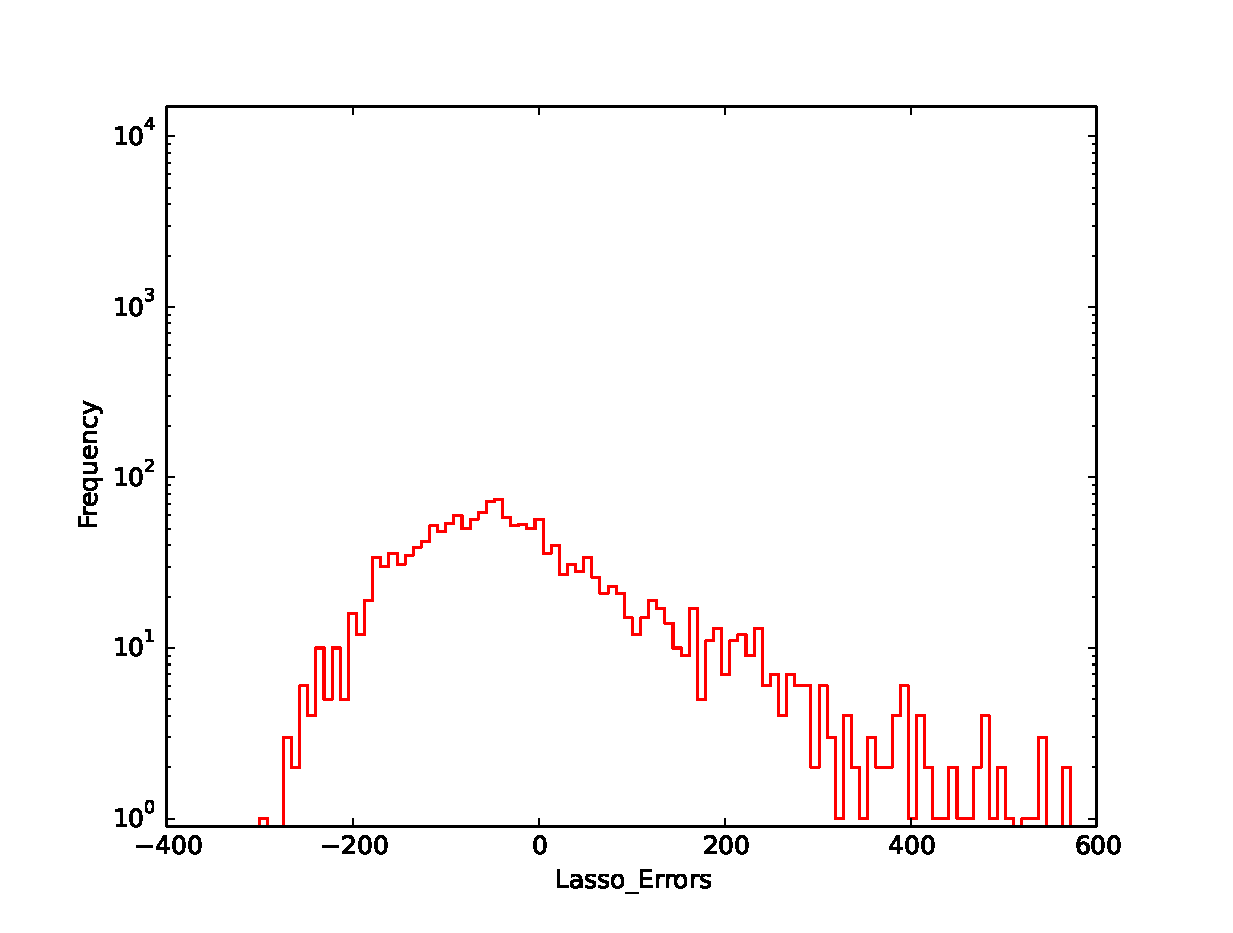
\includegraphics[width=0.6\textwidth]{plots/Lasso_Errors_12.eps}\\
\end{center}
\begin{itemize}
\small
\item{The Lasso algorithms showed greater consistency between KFold and evalution scores, but with worse scores and larger uncertainties than the Random Forest algorithms.}
\item{They also seemed to show a distinct trend to overestimate bike usage (plot on right shows true-predicted).}
\end{itemize}
\end{frame}


%%%%%%%%%%%%%%%%%%%%%%%%%%%%%%%%%%%%%%%%%%%%%%%%%%%%%%%

\begin{frame}{Lasso vs. Random Forest}
\begin{center}
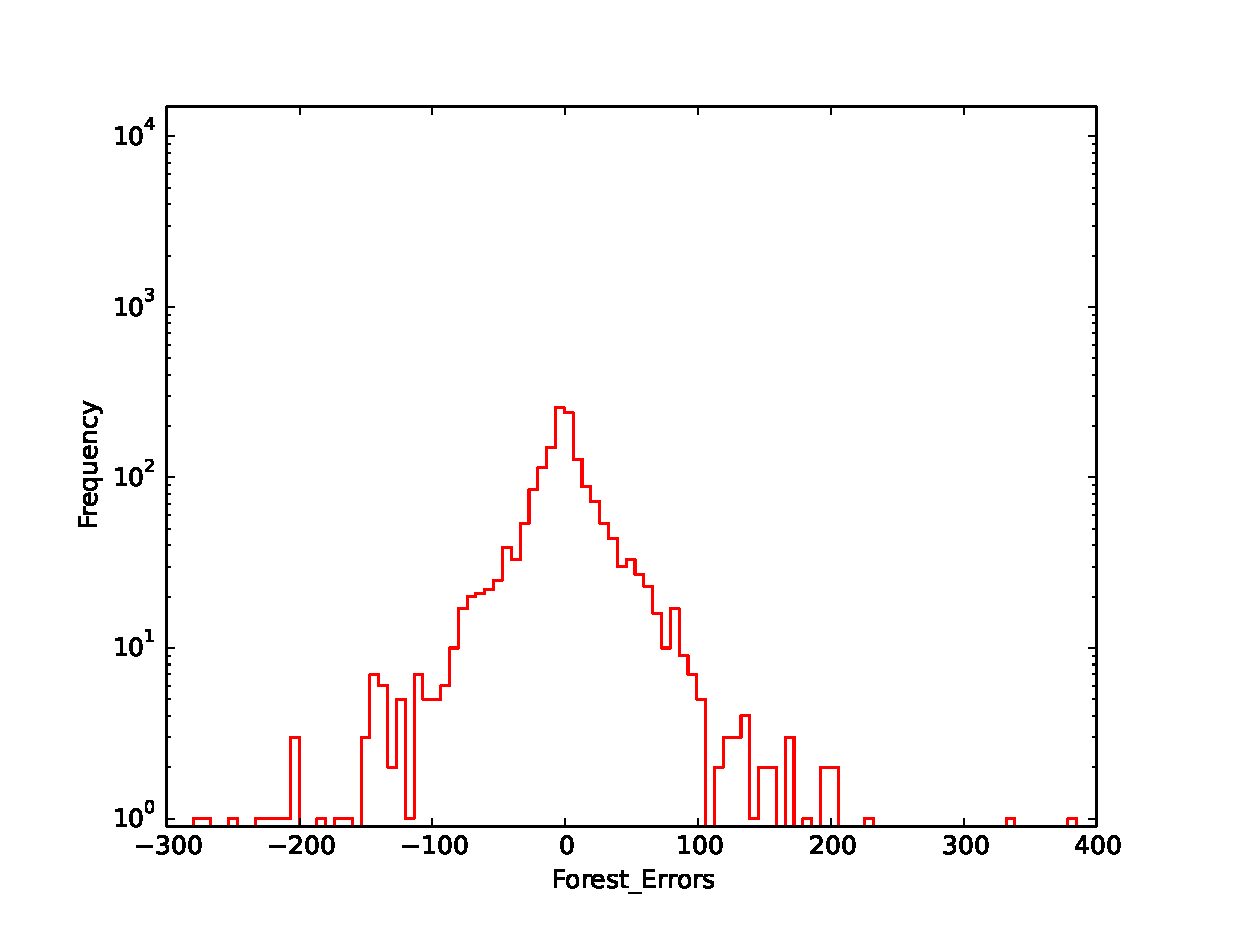
\includegraphics[width=0.6\textwidth]{plots/Forest_Errors_12.eps}
\end{center}
\begin{itemize}
\small
\item{The Random Forest algorithms produced better overall scores with smaller standard deviations and shows a symmetric error distribution (right).  However, for a given algorithm the differences between best KFold, global, and evaluation scores were between 2-4 standard deviations, hinting at possible over-training.}
\item{Both distributions hint that outliers might be present.}
\item{Table for numeric comparison is in the backup slides.}
\end{itemize}
\end{frame}

%%%%%%%%%%%%%%%%%%%%%%%%%%%%%%%%%%%%%%%%%%%%%%%%%%%%%%%

\begin{frame}{Conclusions}
\begin{itemize}
\item{Both the Lasso and Random Forest algorithms were used to build regressors to predict the number of rented bicycles, with an approximate error of 100 bicycles for Lasso and 50 for Random Forest.  The random forest algorithms seemed to perform better but may have been over-trained.}
\item{Expansions:}
\begin{enumerate}
\small
\item{Further exploration of input variables for correlations and redundencies.  Was removing the registered users variable truely necessary?  Assuming that users register somewhat in advance, that information would be suitable for inclusion as an input, and would almost certainly improve the performance.}
\item{Outlier identification.  These preliminary results indicate outliers might well be present, perhaps due to extreme weather conditions such as Hurricane Sandy.  A method for identifying and possible removing these should be developed.}
\item{Exploration of more algorithms and a larger parameter space would also be beneficial.}
\end{enumerate}
\end{itemize}
\end{frame}

%%%%%%%%%%%%%%%%%%%%%%%%%%%%%%%%%%%%%%%%%%%%%%%%%%%%%%%

\begin{frame}{Back-Up}
\end{frame}

%%%%%%%%%%%%%%%%%%%%%%%%%%%%%%%%%%%%%%%%%%%%%%%%%%%%%%%

\begin{frame}{Variable Scatter Plots}
\begin{center}
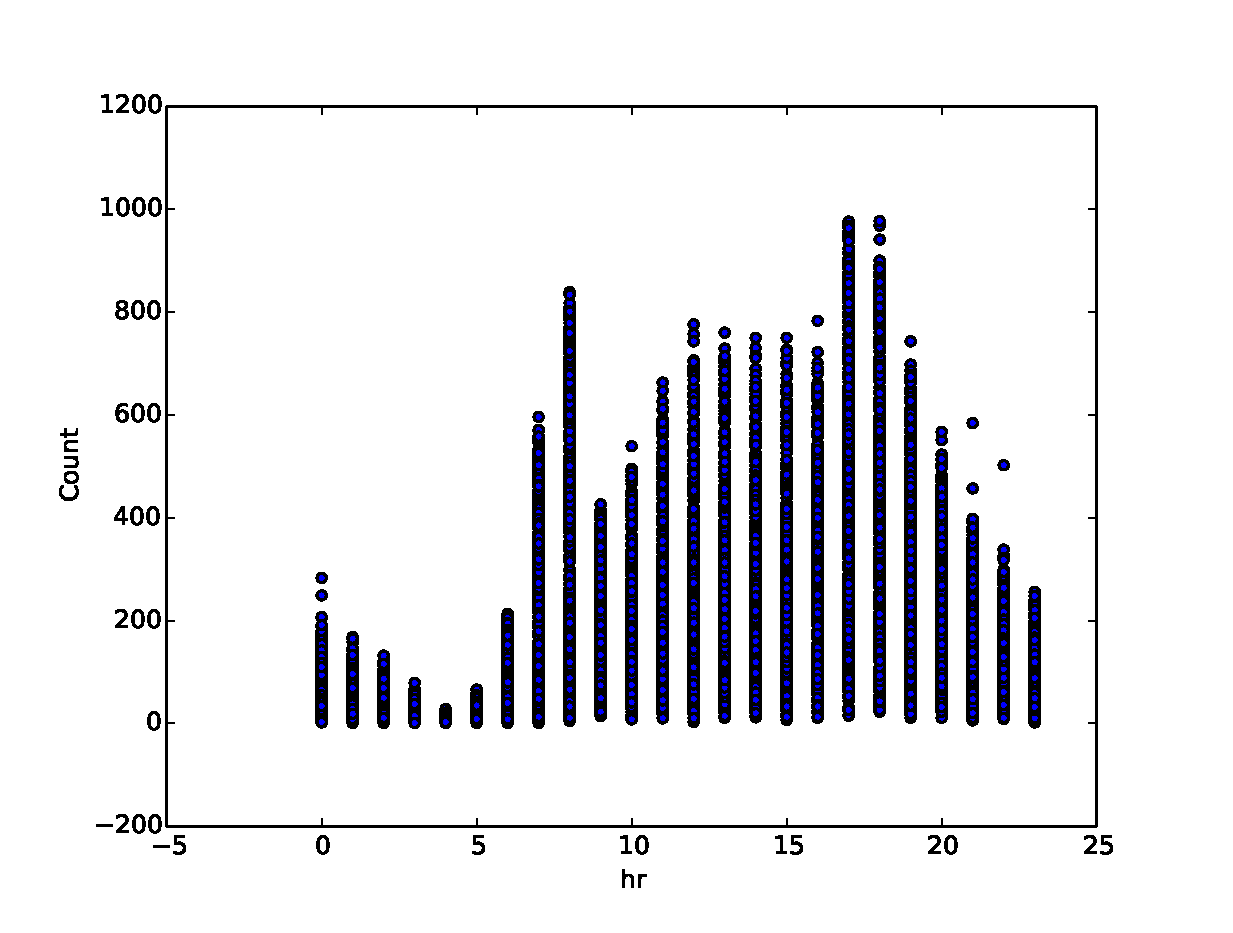
\includegraphics[width=0.35\textwidth]{plots/hr_v_Count_corrcheck.eps}
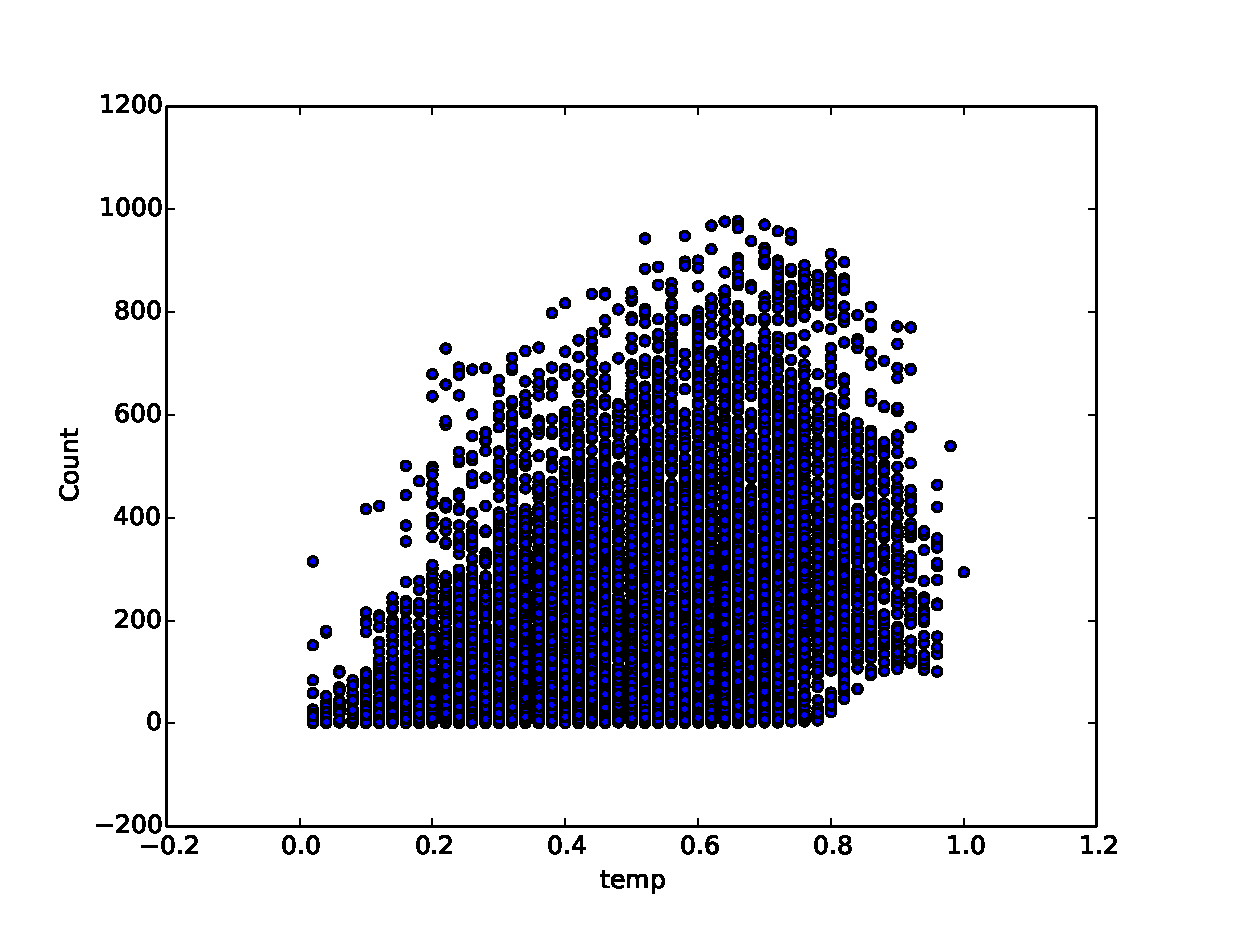
\includegraphics[width=0.35\textwidth]{plots/temp_v_Count_corrcheck.eps}
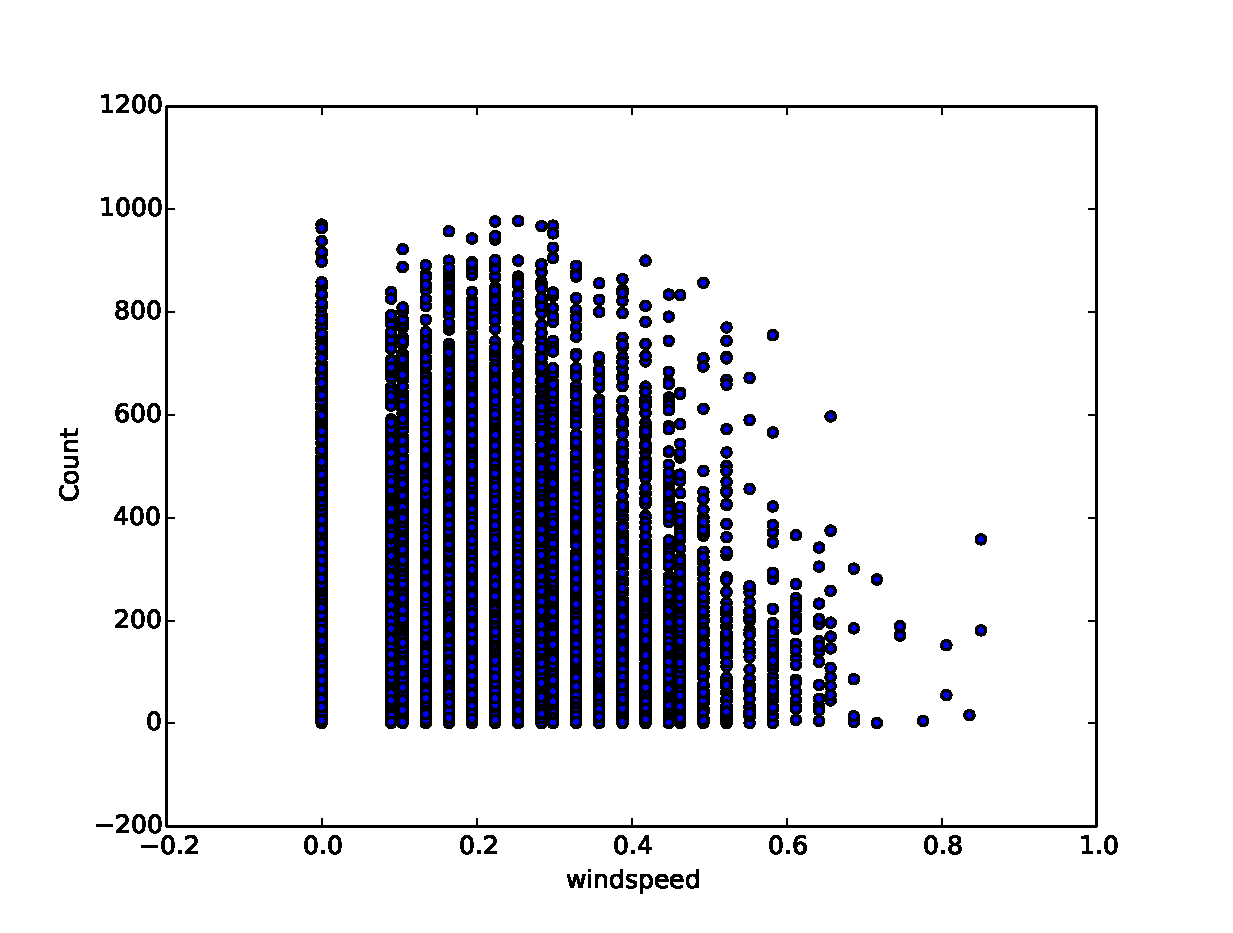
\includegraphics[width=0.35\textwidth]{plots/windspeed_v_Count_corrcheck.eps}\\
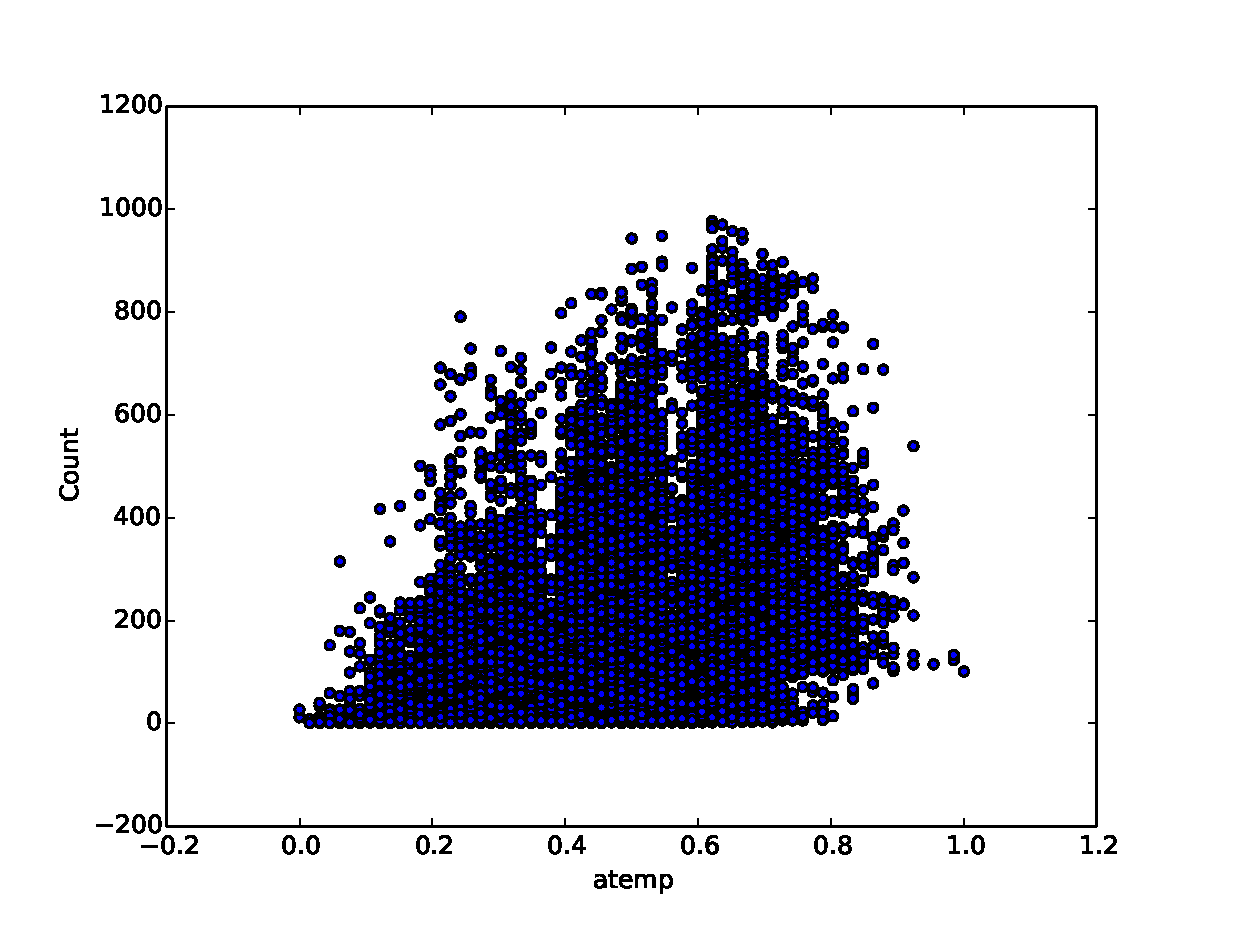
\includegraphics[width=0.35\textwidth]{plots/atemp_v_Count_corrcheck.eps}
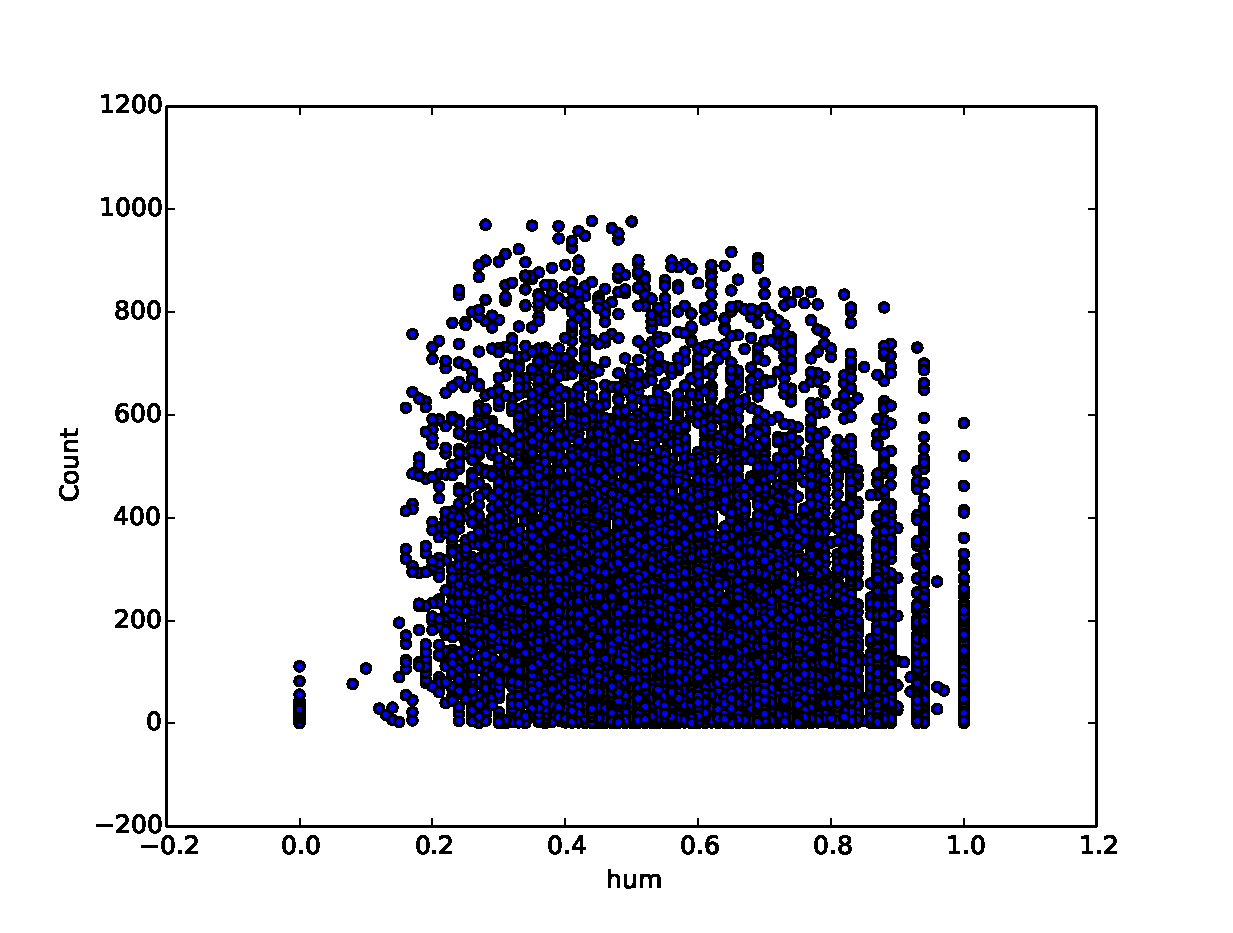
\includegraphics[width=0.35\textwidth]{plots/hum_v_Count_corrcheck.eps}
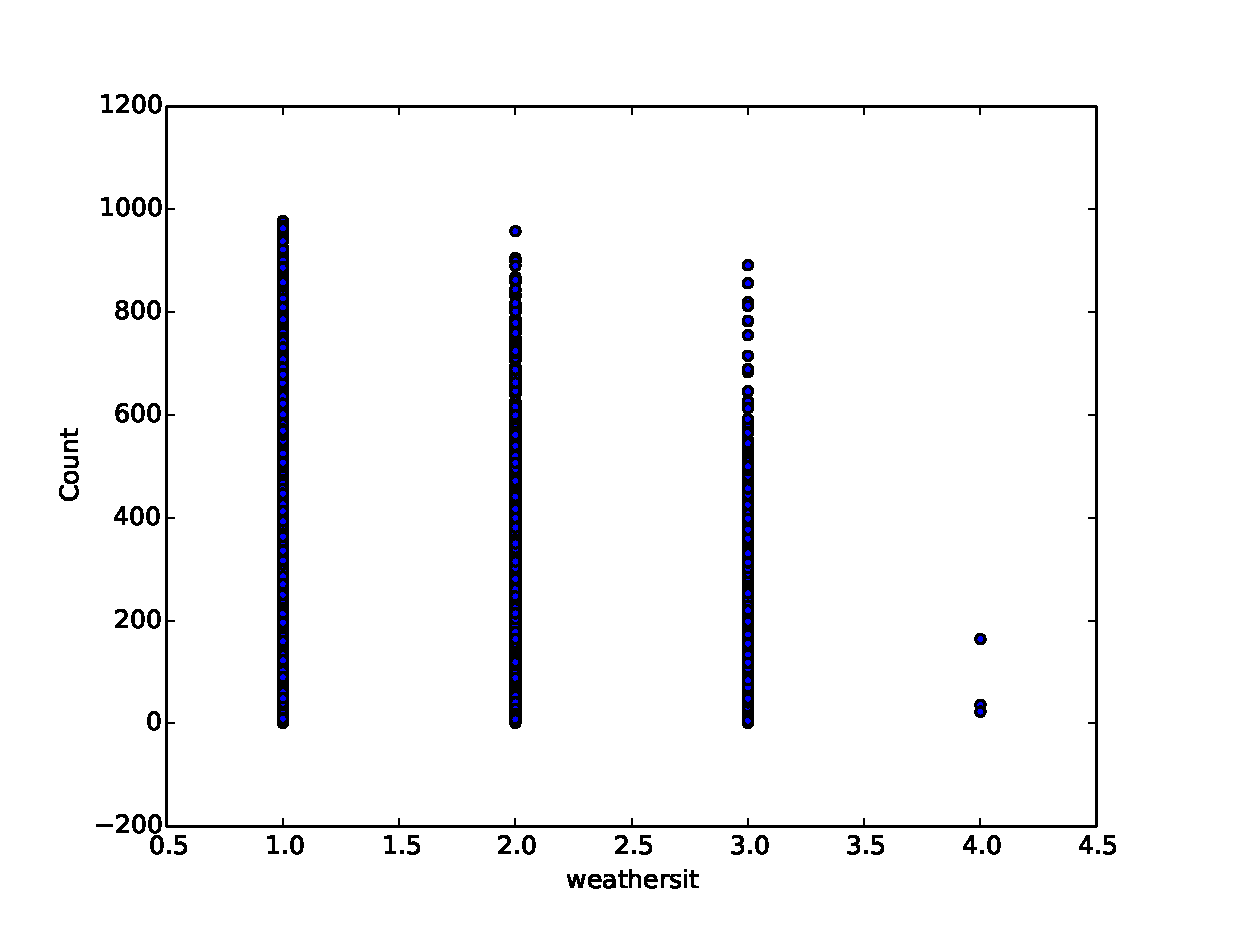
\includegraphics[width=0.35\textwidth]{plots/weathersit_v_Count_corrcheck.eps}\\
\end{center}
\end{frame}

%%%%%%%%%%%%%%%%%%%%%%%%%%%%%%%%%%%%%%%%%%%%%%%%%%%%%%%

\begin{frame}{Variable Scatter Plots (page 2)}
\begin{center}
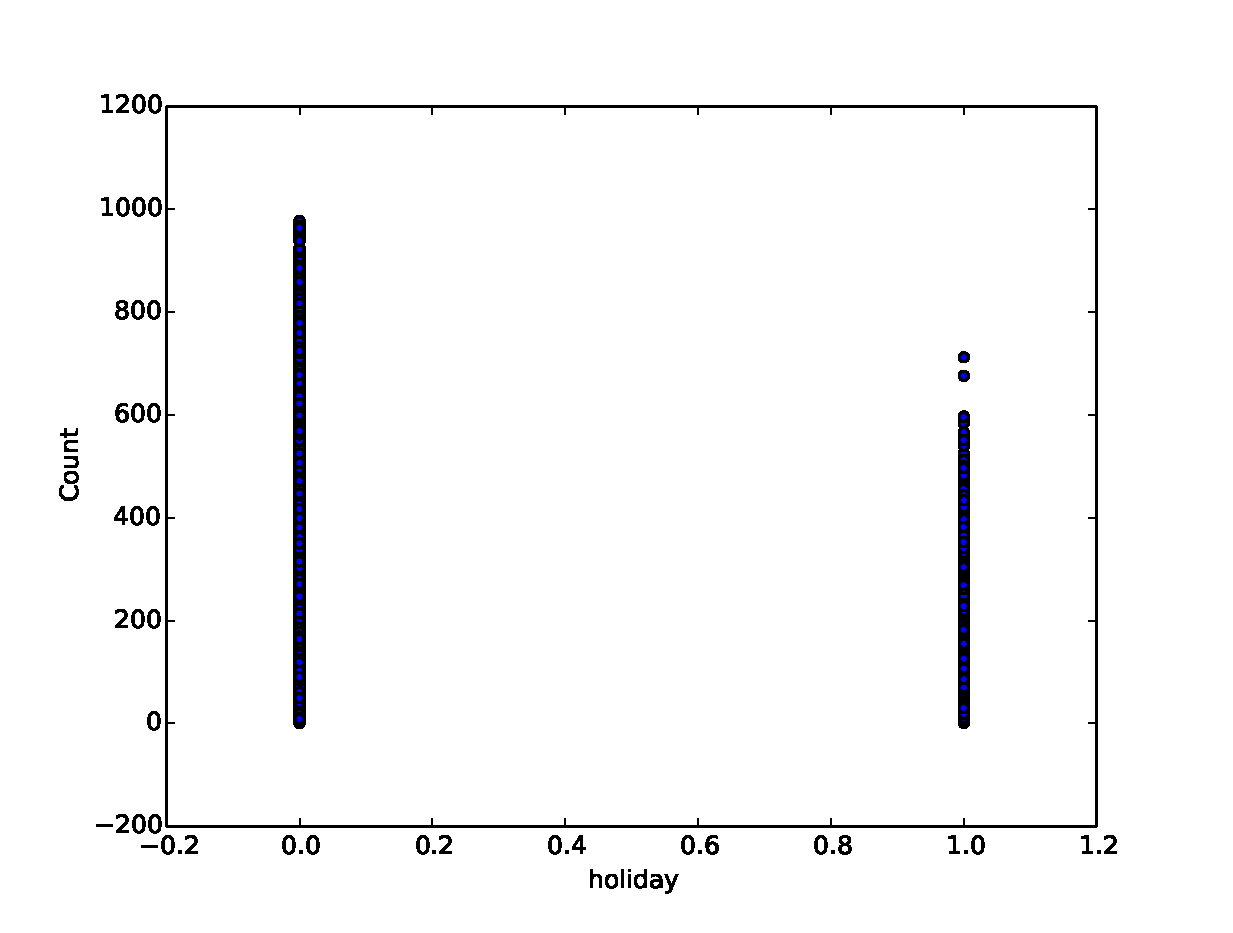
\includegraphics[width=0.35\textwidth]{plots/holiday_v_Count_corrcheck.eps}
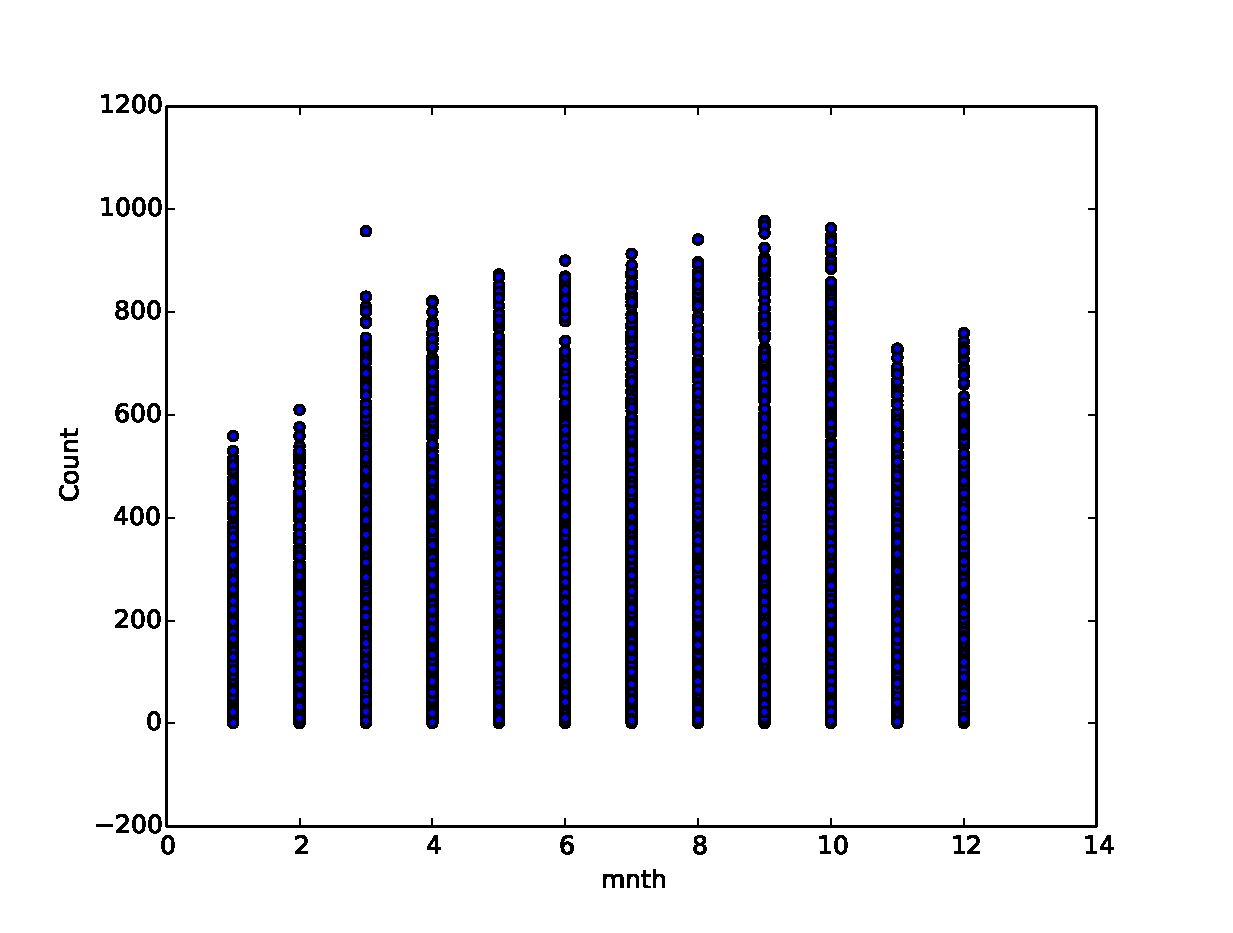
\includegraphics[width=0.35\textwidth]{plots/mnth_v_Count_corrcheck.eps}
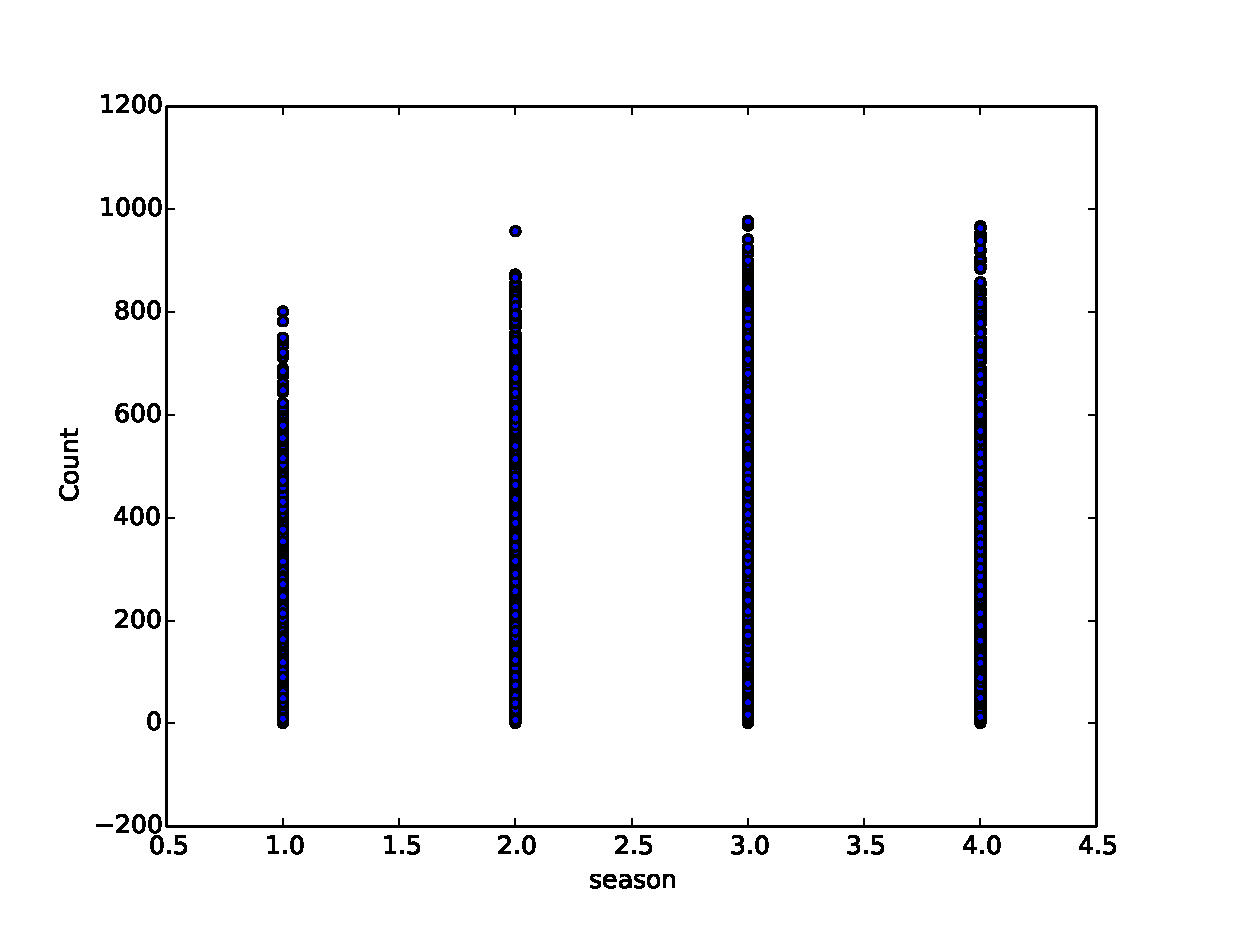
\includegraphics[width=0.35\textwidth]{plots/season_v_Count_corrcheck.eps}\\
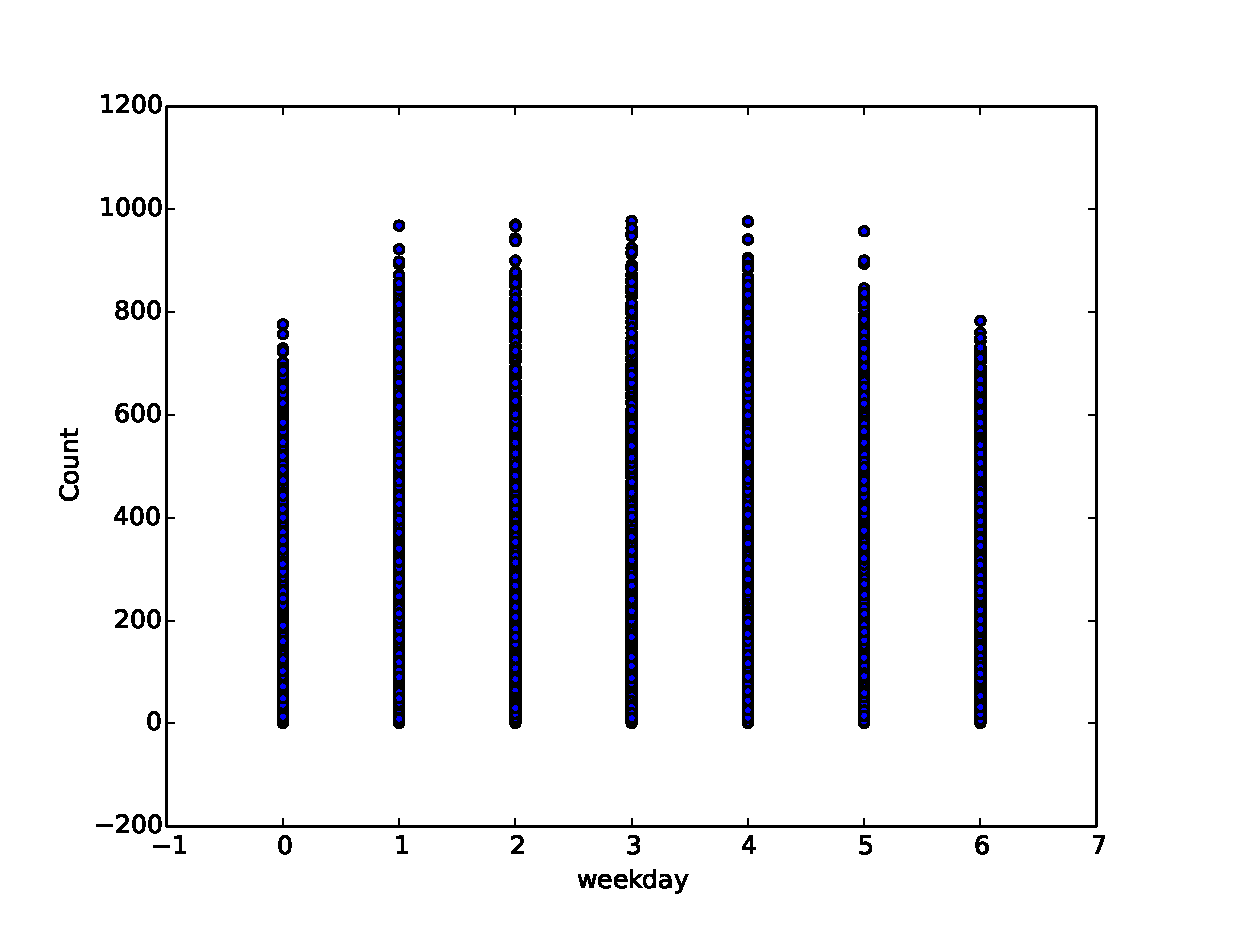
\includegraphics[width=0.35\textwidth]{plots/weekday_v_Count_corrcheck.eps}
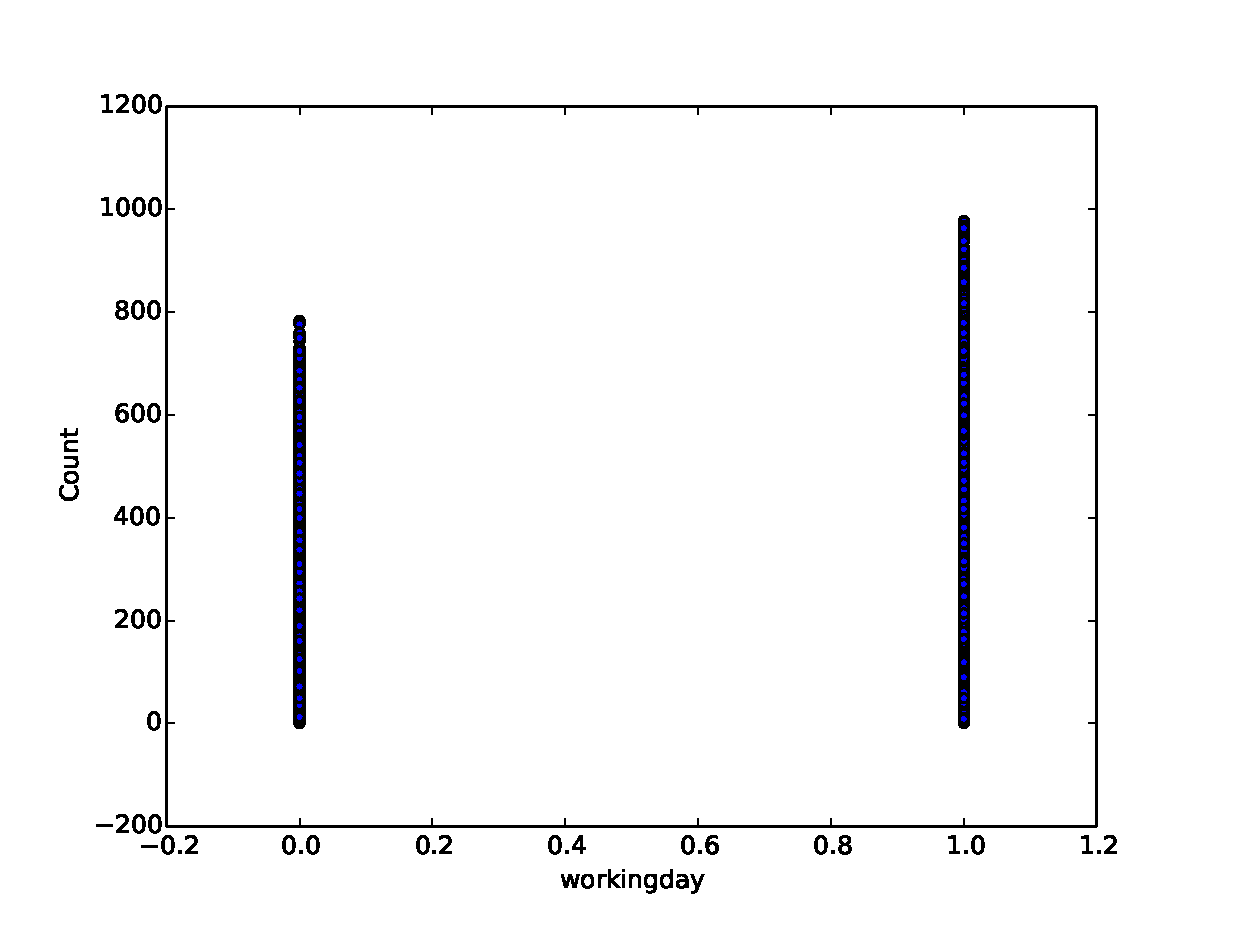
\includegraphics[width=0.35\textwidth]{plots/workingday_v_Count_corrcheck.eps}
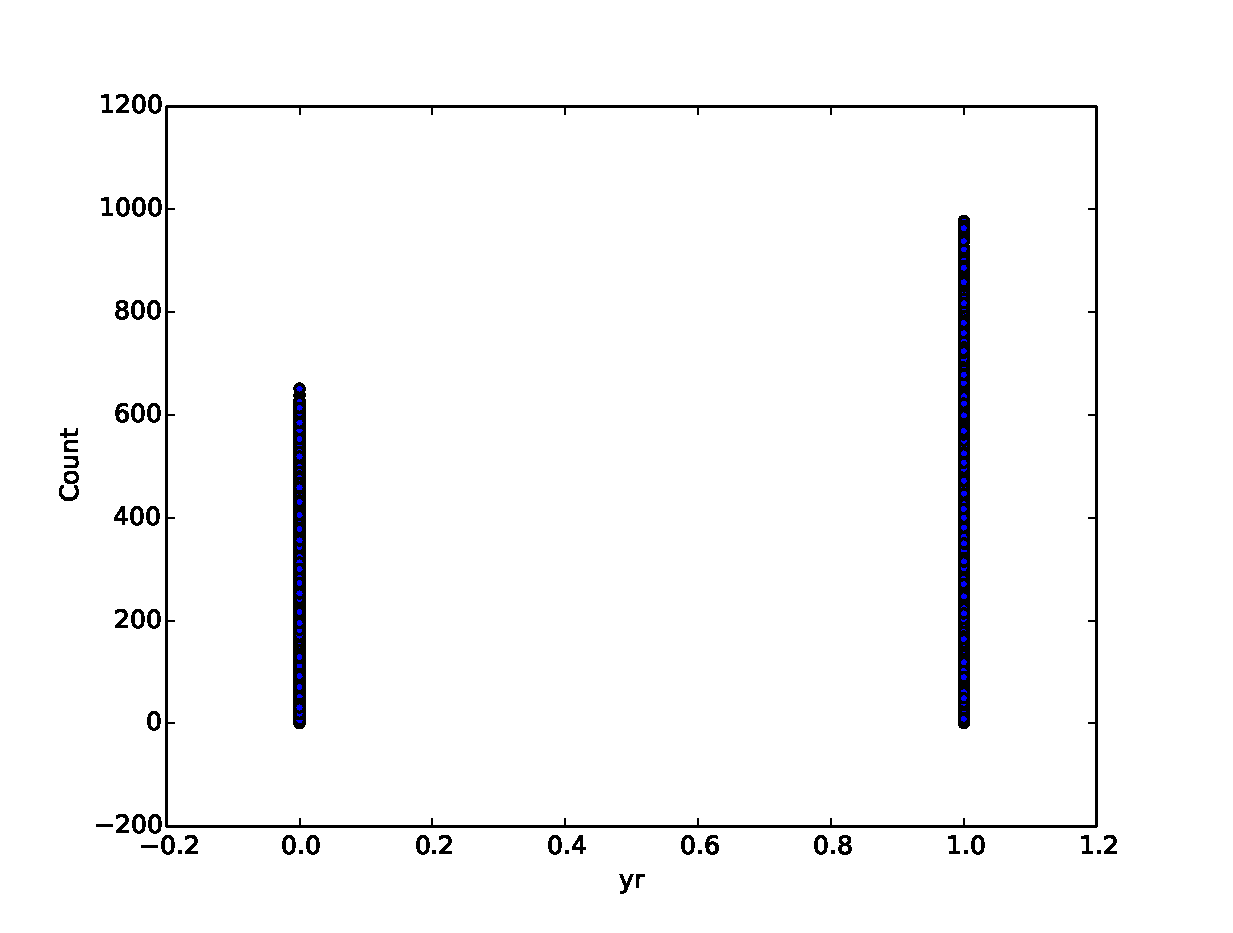
\includegraphics[width=0.35\textwidth]{plots/yr_v_Count_corrcheck.eps}\\
\end{center}
\end{frame}

%%%%%%%%%%%%%%%%%%%%%%%%%%%%%%%%%%%%%%%%%%%%%%%%%%%%%%%

\begin{frame}{Algorithm Comparison}
\begin{center}
\scalebox{0.7}{
\begin{tabular}{|l|c|c|c|}
\hline
& \multicolumn{3}{c|}{Lasso Regression}\\
Variables & 6 & 9 & 12\\
$\alpha$ & 1.0 & 1.0 & 1.0 \\
Best KFold Score & -109.38 $\pm$ 28.26 & -109.51$\pm$28.37 & -109.62$\pm$28.34 \\
Global Score & -106.11 & -106.11 & -106.14 \\
Evaluation Score & -105.42 & -105.43 & -105.48 \\
\hline
 & \multicolumn{3}{c|}{Random Forest Regression}\\
Variables & 6 & 9 & 12 \\
min\_sample\_split & 14 & 10 & 6\\
estimators & 100 & 100 & 100 \\
max\_depth & 12 & 12 & 12 \\
Best KFold Score & -66.87$\pm$15.05 & -66.71$\pm$11.77  & -43.68$\pm$5.54 \\
Global Score & -49.90 & -46.06 & -20.57 \\
Evaluation Score & -58.93 & -56.84 & -28.98 \\
\hline
\end{tabular}
}
\end{center}
\end{frame}

%%%%%%%%%%%%%%%%%%%%%%%%%%%%%%%%%%%%%%%%%%%%%%%%%%%%%%%

\begin{frame}{Error Comparison)}
\begin{center}
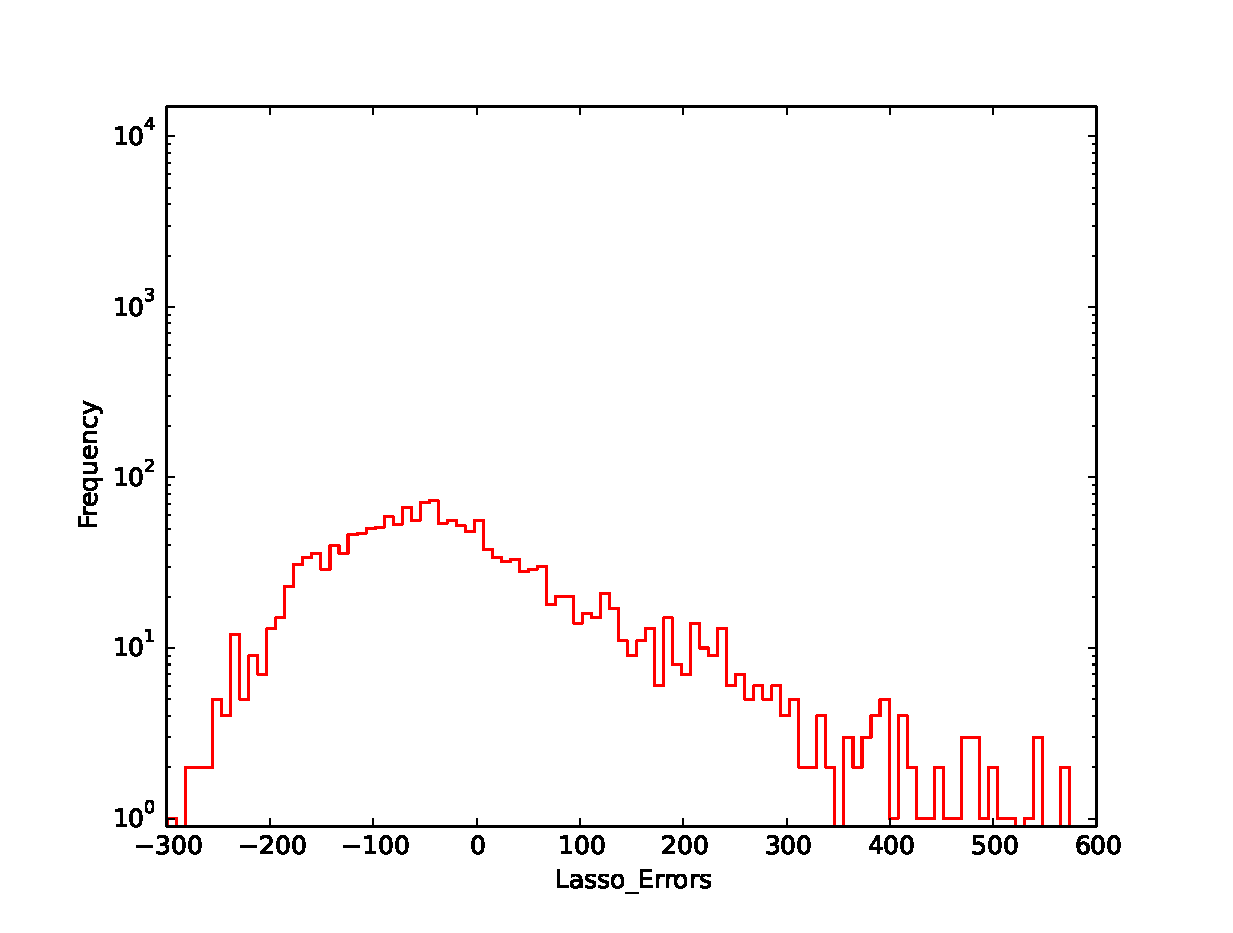
\includegraphics[width=0.35\textwidth]{plots/Lasso_Errors_6.eps}
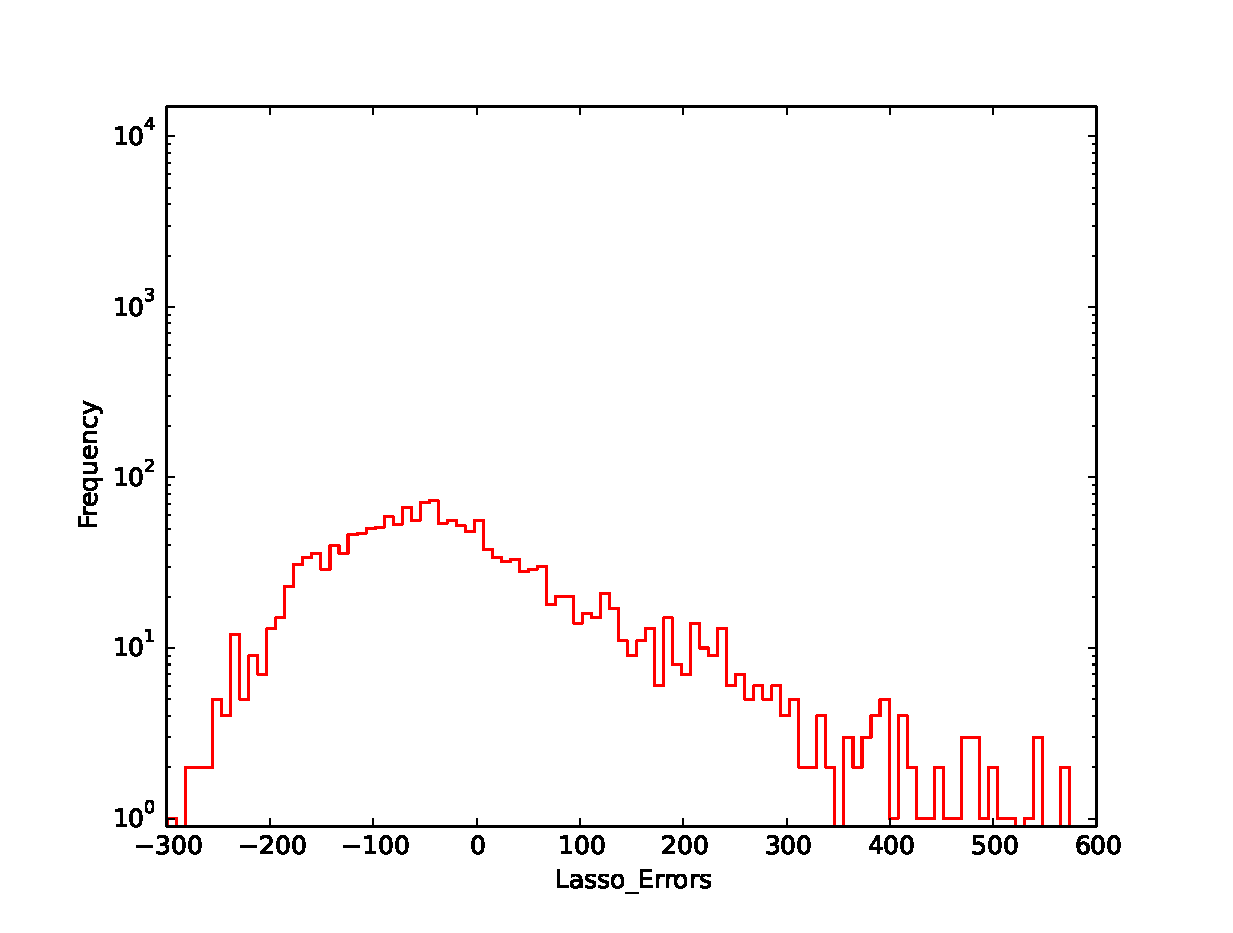
\includegraphics[width=0.35\textwidth]{plots/Lasso_Errors_9.eps}
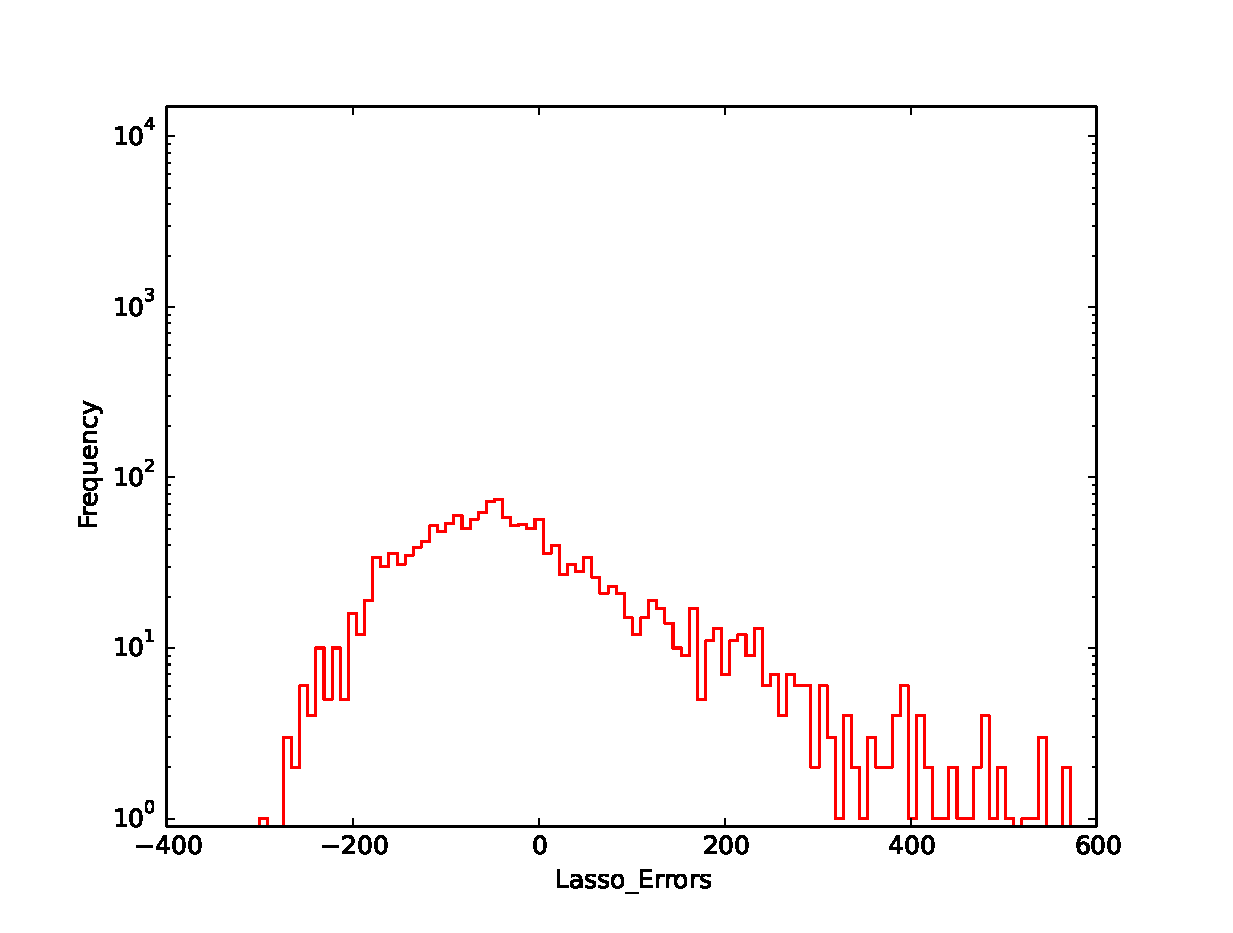
\includegraphics[width=0.35\textwidth]{plots/Lasso_Errors_12.eps}\\
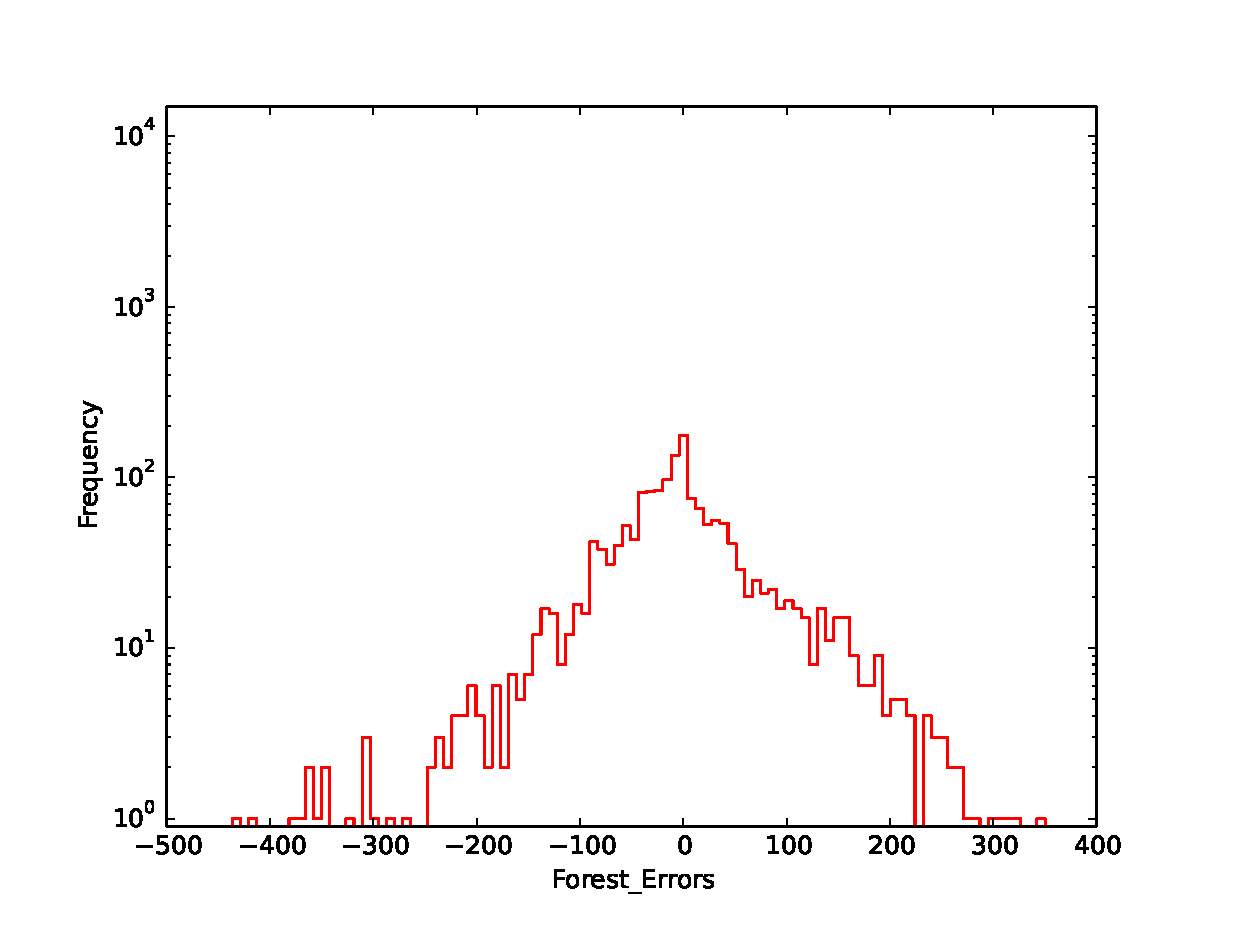
\includegraphics[width=0.35\textwidth]{plots/Forest_Errors_6.eps}
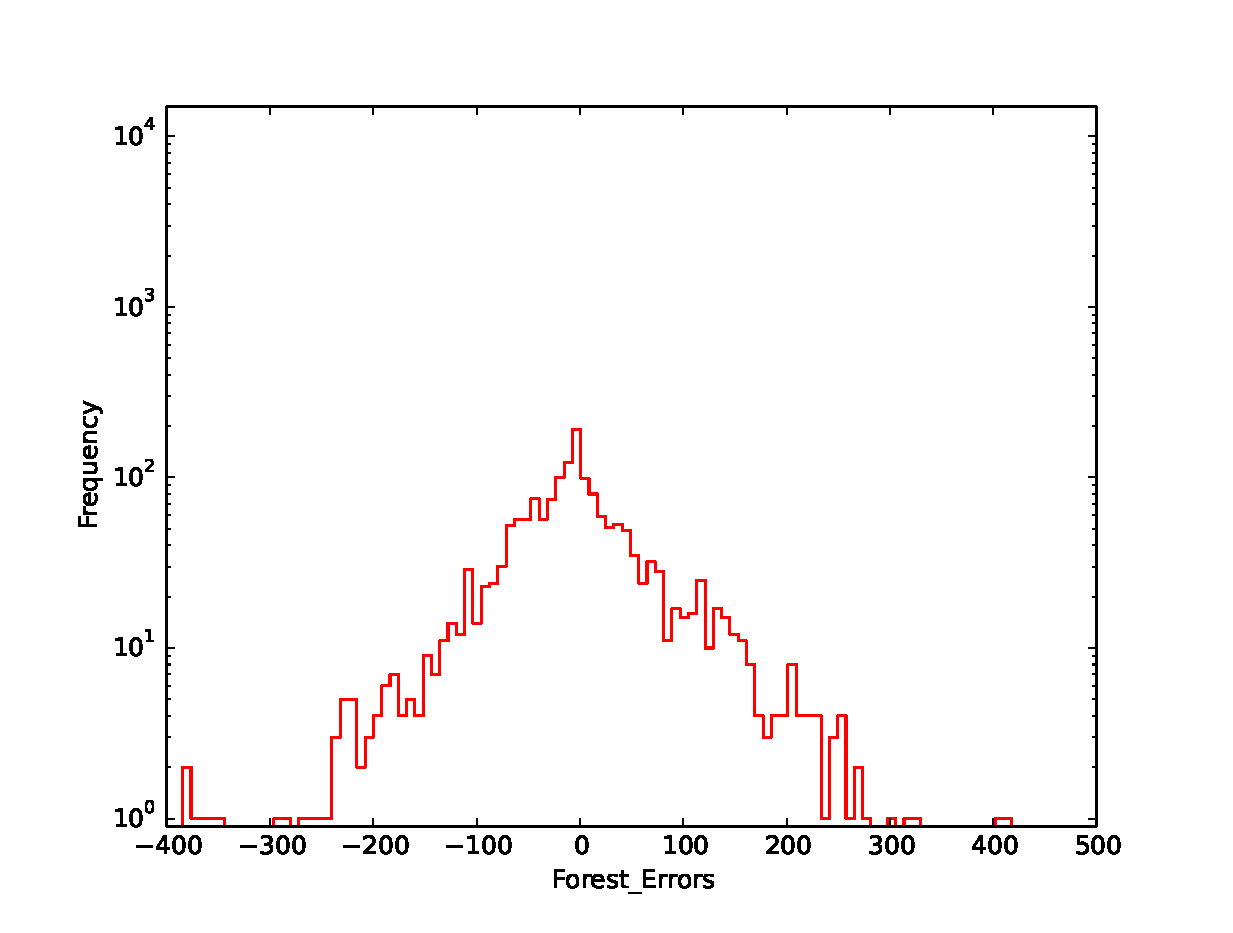
\includegraphics[width=0.35\textwidth]{plots/Forest_Errors_9.eps}
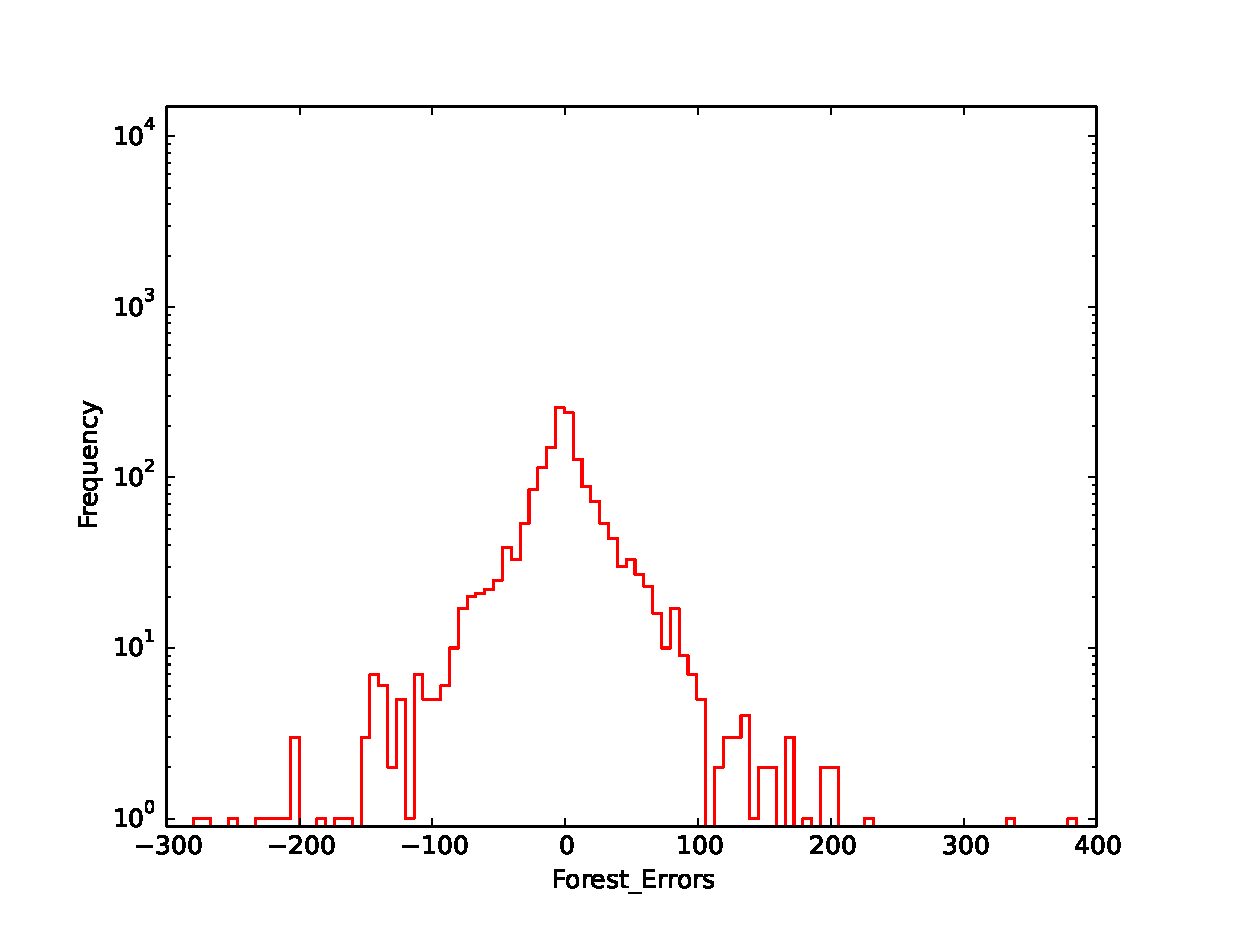
\includegraphics[width=0.35\textwidth]{plots/Forest_Errors_12.eps}\\
\end{center}
\tiny Left column is for algorithms with six input variables, center has nine, and right has all twelve.
\end{frame}

%%%%%%%%%%%%%%%%%%%%%%%%%%%%%%%%%%%%%%%%%%%%%%%%%%%%%%%


\end{document}
